\section{Modeling Approaches}
\label{sec:24_modeling_approaches}

The co-simulation framework developed in this thesis integrates subsystem models from three modeling approaches at distinct abstraction levels.
This section characterizes each approach at the level needed to understand the component abstractions in Chapter~\ref{chap:architecture}, the wrapper implementations in Chapter~\ref{chap:implementation}, and the model configurations
used in the case study (Chapter~\ref{chap:case_study}).
The selection and justification of the specific tools used for each approach is given in Chapter~\ref{chap:requirements}.

%%%%%%%%%%%%%%%%%%%%%%%%%%%%%%%%%%%%%%%%%
\subsection{Equation-Based Modeling}
\label{sec:241_modeling_equation_based}

Section~\ref{sec:intro_sota} introduced equation-based modeling as a compact way to describe lumped-parameter multi-domain subsystems, and Section~\ref{sec:21_continuous_time} formalized the underlying mathematical representation.
This subsection bridges the two views. It shows how such a mathematical formulation is expressed in a concrete modeling language and how the resulting source model is translated into an executable simulation unit that the co-simulation framework can consume.
We use the pendulum introduced in Section~\ref{sec:211_dynamical_systems} as a running example and the Modelica language~\cite{Modelica_Fritzson} as a representative for this modeling approach.

\paragraph{Modelica Realization.}
Listing~\ref{lst:modelica_pendulum} shows a minimal Modelica realization of the pendulum.
The model declares the physical parameters $m$, $L$, and $J$, the gravitational constant $g$, and the initial conditions $\theta_0$ and $\omega_0$.
Its interface consists of the input torque $\tau$ and the two outputs $\theta$ and $\omega$.
The \texttt{equation} section states the two ordinary differential equations already given in Equation~\eqref{eq:pendulum_ode} without prescribing a computational direction.

\begin{listing}[htbp]
\begin{lstlisting}[style=modelica]
model Pendulum
  parameter Real m(unit="kg")          "Pendulum mass";
  parameter Real L(unit="m")           "Hinge to center of mass";
  parameter Real I(unit="kg.m2")       "Moment of inertia about pivot";
  parameter Real theta_0(unit="rad")   "Initial angle";
  parameter Real omega_0(unit="rad/s") "Initial angular velocity";
  constant  Real g(unit="m/s2")        "Gravitational accel.";

  Modelica.Blocks.Interfaces.RealInput  tau(unit="N.m");
  Modelica.Blocks.Interfaces.RealOutput theta(unit="rad");
  Modelica.Blocks.Interfaces.RealOutput omega(unit="rad/s");

initial equation
  theta = theta_0;
  omega = omega_0;

equation
  der(theta) = omega;
  der(omega) = (tau - m * g * L * sin(theta)) / I;
end Pendulum;
\end{lstlisting}
\caption{Minimal Modelica realization of the pendulum from Section~\ref{sec:211_dynamical_systems}. Values are omitted.}
\label{lst:modelica_pendulum}
\end{listing}

Each declaration in Listing~\ref{lst:modelica_pendulum} corresponds to a quantity of the state-space form of Section~\ref{sec:211_dynamical_systems}, grouped by variability.
Constants such as $g$ are universal physical quantities and cannot be modified.
Parameters such as $m$, $L$, and $J$ are design values that must be assigned before initialization and stay fixed during a run as they are not part of the state (Section~\ref{sec:211_dynamical_systems}).
Variables are time-dependent quantities and cover the state, input, and output components of the state-space form.
In Listing~\ref{lst:modelica_pendulum}, the state is $(\theta,\,\omega)$, the input is $\tau$, and the outputs are $\theta$ and $\omega$.

\paragraph{Translation Pipeline.}
The \texttt{equation} section states relations between variables rather than assignments.
Although \texttt{der(theta) = omega} looks like an assignment, Modelica treats it as an equality that the tool may sort in either direction.
The computational direction of the equations is therefore a property of the translated model, not of the source code.
At the source level, the only directed elements are the declared \texttt{RealInput} and \texttt{RealOutput} ports, which fix the external interface independently of the internal equation causality.

The translation from a source model like Listing~\ref{lst:modelica_pendulum} to an executable simulation unit proceeds in three conceptual stages~\cite{Modelica_Fritzson}.
In the first stage, the modeling tool flattens the source.
The class hierarchy is resolved and connect statements are rewritten as algebraic equations, leaving a flat system of differential and algebraic equations without any remaining object-oriented structure.
In the second stage, structural analysis is performed on this flat system.
A computational direction is assigned to each variable and the equations are sorted along their dependencies into a block-lower-triangular form.
When the flat system is a high-index DAE of the kind introduced in Section~\ref{sec:212_ode_dae}, symbolic index reduction is applied before causalization.
In the third stage, the sorted equations are translated into generated code and linked with a numerical solver.
The resulting unit has a fixed signal-level interface, an embedded solver, and a direct feedthrough structure (Section~\ref{sec:213_direct_feedthrough}) that is fixed once at translation time.
This unit is packaged as a Functional Mock-up Unit (Section~\ref{sec:237_cosim_fmi}) for use in the co-simulation framework.

\paragraph{Simulation Unit Contract}
When the translated unit is used in a co-simulation scenario, the simulation-unit lifecycle introduced in Section~\ref{sec:232_cosim_formulation} governs in which phase each variable may be read or written.
The access rules follow directly from the Modelica variability classes of Listing~\ref{lst:modelica_pendulum}.
Constants are fixed and never settable.
Parameters are writable during the configuration and initialization phases and are frozen once advancement begins.
Inputs are writable at each communication point during advancement.
Outputs are read-only and are refreshed at the end of each communication step.
Internal variables outside the declared interface are not part of the contract.

The direct feedthrough structure fixed at translation time is exposed as contract metadata that the master algorithm can query before the first step, providing the relation $F_i$ defined in Section~\ref{sec:232_cosim_formulation}.
A simulation unit may additionally expose operations to snapshot and restore its full internal state, which enables the rollback required by the hybrid event protocol of Section~\ref{sec:236_cosim_hybrid}.
The Functional Mock-up Interface in Co-Simulation mode (Section~\ref{sec:237_cosim_fmi}) standardizes this contract through a fixed set of operators for configuration, initialization, stepping, and state access.
The wrapper implementation in Section~\ref{sec:impl_fmu} invokes these operators through the \texttt{fmpy} library and maps them onto the component abstractions of the framework.

%%%%%%%%%%%%%%%%%%%%%%%%%%%%%%%%%%%%%%%%%
\subsection{Musculoskeletal Modeling}
\label{sec:242_modeling_musculoskeletal}

Section~\ref{sec:intro_sota} introduced musculoskeletal modeling as a domain-specific approach for systems which interact with the human body.
This subsection describes how a musculoskeletal model is structured, what additional dynamics it introduces beyond the lumped-parameter formulations of Section~\ref{sec:21_continuous_time}, and how such a model is turned into a simulation unit for co-simulation.
We use OpenSim~\cite{OpenSim_Delp,seth_opensim_2018} as the representative tool and its underlying multibody engine Simbody~\cite{sherman_simbody_2011} as the computational back-end.
The pendulum of Section~\ref{sec:211_dynamical_systems} serves again as a running example, now formulated as a multibody model.

\paragraph{Multibody Topology.}
A multibody model is defined by its topology where rigid bodies are arranged in a tree structure and are connected by joints.
Each joint introduces one or more generalized coordinates that describe the relative motion between two bodies.
Figure~\ref{fig:opensim_pendulum_topology} shows the topology of the pendulum modeled in OpenSim.
The generalized coordinate of this joint is the pendulum angle~$\theta$, which corresponds to the state variable introduced in Section~\ref{sec:211_dynamical_systems}.
Physical properties such as mass, center of mass, and moment of inertia are attached to each body.

\begin{figure}[htbp]
    \centering
    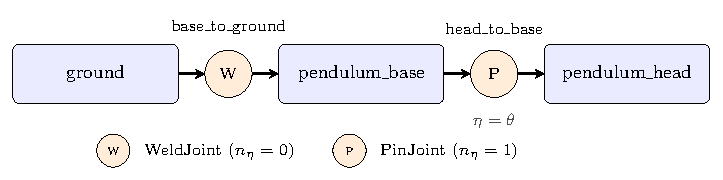
\includegraphics[width=\textwidth]{figures/2_theoretical_background/multibody_topology.pdf}
    \caption{Multibody topology of the pendulum modeled in OpenSim.
             The ground body is rigidly attached to \texttt{pendulum\_base}
             via a weld joint.
             A pin joint connects \texttt{pendulum\_base} to
             \texttt{pendulum\_head} and introduces the single
             generalized coordinate~$\theta$.}
    \label{fig:opensim_pendulum_topology}
\end{figure}

\paragraph{Equations of Motion.}
A multibody model formulated in generalized coordinates
$q \in \mathbb{R}^{n_q}$ leads to a second-order ODE of the form
\begin{equation}
    \ddot{q}
    = M(q)^{-1}
      \bigl\{
        \tau
        - C(q,\dot{q})
        - G(q)
        + F
      \bigr\},
    \label{eq:multibody_eom}
\end{equation}
where $M(q)$ is the configuration-dependent mass matrix, $C$ collects velocity-dependent (Coriolis and centrifugal) forces, $G$ collects gravitational forces, $\tau$ denotes joint torques, and $F$ represents external generalized forces~\cite{OpenSim_Delp,seth_opensim_2018}.
For the pendulum of Figure~\ref{fig:opensim_pendulum_topology}, the single generalized coordinate $q = \theta$ reduces Equation~\eqref{eq:multibody_eom} to a scalar form.
The mass matrix becomes the scalar moment of inertia~$I$, the Coriolis term vanishes, and the gravitational term reduces to $mgL\sin\theta$.
The result is the pendulum ODE already stated in Equation~\eqref{eq:pendulum_ode}.
In state-space form with $x = [q,\,\dot{q}]^\top$, Equation~\eqref{eq:multibody_eom} is an ODE system of the kind introduced in Section~\ref{sec:211_dynamical_systems}.

\paragraph{Forces and Actuation.}
OpenSim models support several types of forces that act on the multibody system.
Passive forces include springs, dampers, and contact models such as the Hunt--Crossley model, which computes contact forces from the overlap of contact geometries attached to bodies.
Ideal actuators apply forces or torques that are directly proportional to a scalar control input.
The pendulum model used in this thesis employs a \texttt{CoordinateActuator} of this kind, which applies a torque directly along the joint axis of~$\theta$.
Muscle actuators are the most complex force elements.
Each muscle is modeled as a path between attachment points on rigid bodies and generates a force that depends on its current activation~$a$, fibre length~$l$, and fibre contraction velocity~$\dot{l}$.
The resulting muscle forces are mapped to joint torques through configuration-dependent moment arms~$R(q)$.

\paragraph{Forward Dynamics.}
Forward dynamics computes the time evolution of a musculoskeletal model from a given initial state and a time history of control inputs.
The generalized accelerations follow from Equation~\eqref{eq:multibody_eom}, where the joint torques due to muscles are
\begin{equation}
    \tau_m = R(q)\,f(a,\,l,\,\dot{l}).
    \label{eq:muscle_torque}
\end{equation}
The muscle states evolve according to their own dynamics.
Activation~$a$ is governed by a first-order excitation-to-activation model driven by a neural excitation signal~$e \in [0,1]$:
\begin{equation}
    \dot{a} = A(a,\,e).
    \label{eq:activation_dynamics}
\end{equation}
Fibre length~$l$ evolves according to a contraction model that couples the muscle to the skeletal configuration:
\begin{equation}
    \dot{l} = \Lambda(a,\,l,\,q,\,\dot{q}).
    \label{eq:contraction_dynamics}
\end{equation}
The full state vector of a musculoskeletal model is therefore
$x = [q,\,\dot{q},\,a,\,l]^\top$~\cite{OpenSim_Delp}.
For models that use only ideal actuators, the muscle states are absent and the state reduces to $x = [q,\,\dot{q}]^\top$.
Forward dynamics integrates this ODE system numerically, producing trajectories of all state variables over the simulation horizon.
This is in contrast to inverse dynamics, which takes a known motion as input and computes the joint torques required to produce it~\cite{OpenSim_Delp,seth_opensim_2018}.

\paragraph{Runtime Architecture.}
OpenSim delegates all dynamics computations to the Simbody multibody engine~\cite{sherman_simbody_2011}.
At runtime, three objects cooperate.
The \emph{Model} encapsulates the system definition, including bodies, joints, forces, and muscles.
It is itself stateless and remains unchanged during a simulation.
The \emph{State} holds everything that changes over time.
This includes the current time~$t$, the generalized coordinates~$q$ and velocities~$\dot{q}$, any auxiliary continuous states such as muscle activations and fibre lengths, and discrete variables that are modified only by event handlers.
The \emph{Manager} couples Model and State and drives a numerical integrator to advance the state through time.

Simbody organizes derived quantities in a staged realization cache inside the State object.
The stages follow a strict dependency order: \emph{Position} (body poses from~$q$), \emph{Velocity} (body velocities from~$\dot{q}$), \emph{Dynamics} (forces from poses, velocities, and muscle states), and \emph{Acceleration} (generalized accelerations from the equations of motion).
Each stage depends on all previous stages.
Requesting a quantity at a given stage triggers the computation of that stage and all earlier stages that have not yet been realized.
When a state variable is modified, the cache is automatically invalidated from the affected stage onward.
For example, changing a generalized speed invalidates the Velocity, Dynamics, and Acceleration stages but preserves already-computed positions.

\paragraph{Simulation-Unit Contract.}
Unlike equation-based models exported through FMI (Section~\ref{sec:241_modeling_equation_based}), musculoskeletal models do not expose a standardized interface descriptor.
There is no machine-readable declaration of variable causality, variability, or direct feedthrough structure.
Which quantities serve as inputs and outputs, how parameters are applied before initialization, and whether state snapshots are feasible all depend on the concrete model and its elements.
A generic wrapper can provide the runtime infrastructure, including the Model--State--Manager lifecycle, the realization calls, and the integrator configuration.
The port specification, parameter mapping, and state-access logic must be supplied by a model-specific subclass.
The wrapper implementation in Section~\ref{sec:impl_opensim} follows this division.

%%%%%%%%%%%%%%%%%%%%%%%%%%%%%%%%%%%%%%%%%
\subsection{Finite Element Modeling}
\label{sec:243_modeling_fem}

Section~\ref{sec:intro_sota} introduced finite element analysis as a way to resolve spatially distributed effects that lumped-parameter models cannot capture.
The equation-based and musculoskeletal approaches of the preceding subsections predict global kinematics and kinetics efficiently but do not resolve quantities within the subsystem geometry.
When local deformation, stress, or distributed contact must be evaluated explicitly, a spatially resolved formulation is required.
Finite element analysis provides this capability by discretizing the geometry into elements and approximating the solution field over that mesh.

This subsection describes how a continuum-mechanical model is cast into a form suitable for time integration and how the resulting simulation unit is embedded in the co-simulation framework.
The pendulum of Section~\ref{sec:211_dynamical_systems} serves again as a running example, now formulated as a deformable body.

\paragraph{Kinematics.}
A body is described by the collection of material points in space.
The reference configuration $\Omage$ of a body describes the initial, undeformed configuration.
A deformation of the body occurs due to external forces acting on the body.
The deformation is described by the function $\phi: \Omega \to \mathbb{R}^3$ and gives the position of the material point $x \in \Omega$ of the reference configuration after deformation.
A displacement describes the difference $u(x) = \phi(x) - x$.
The boundary of a body is denoted by $\partial \Omega$.

\paragraph{Hyperelastic Constitutive Law.}

\paragraph{Stress Measures.}

\paragraph{Variational Formulation and Equilibrium}

\paragraph{}
Let $\Omega \subset \mathbb{R}^d$ with $d \in \{2,3\}$ denote the reference configuration of the body, with boundary $\partial\Omega = \overline{\Gamma_D \cup \Gamma_N}$ and $\Gamma_D \cap \Gamma_N = \emptyset$.
The motion is described by a deformation map $\varphi(\mathbf{X},t) : \Omega \times [0,T] \to \mathbb{R}^d$ and the associated displacement field $\mathbf{u}(\mathbf{X},t) = \varphi(\mathbf{X},t) - \mathbf{X}$.
Differentiation with respect to the reference coordinates yields the deformation gradient
\begin{equation}
  \mathbf{F}(\mathbf{X},t) \;=\; \nabla \varphi \;=\; \mathbf{I} + \nabla \mathbf{u},
  \label{eq:fem_F}
\end{equation}
and the symmetric right Cauchy--Green tensor $\mathbf{C} = \mathbf{F}^\top \mathbf{F}$, from which the Green--Lagrange strain $\mathbf{E} = \tfrac{1}{2}(\mathbf{C} - \mathbf{I})$ follows.

Conservation of linear momentum, expressed in the reference configuration, yields the strong form
\begin{equation}
  \rho_0 \, \ddot{\mathbf{u}} \;=\; \nabla \cdot \mathbf{P} + \mathbf{b}_0
  \qquad \text{in } \Omega \times (0,T],
  \label{eq:fem_strong}
\end{equation}
where $\rho_0$ is the reference mass density, $\mathbf{P}$ the first Piola--Kirchhoff stress, and $\mathbf{b}_0$ a body-force density per unit reference volume.
The formulation is closed by boundary and initial conditions
\begin{equation}
  \mathbf{u} = \hat{\mathbf{u}} \text{ on } \Gamma_D, \qquad
  \mathbf{P} \mathbf{N} = \hat{\mathbf{t}}_0 \text{ on } \Gamma_N, \qquad
  \mathbf{u}(\cdot,0) = \mathbf{u}_0, \quad \dot{\mathbf{u}}(\cdot,0) = \mathbf{v}_0,
  \label{eq:fem_bcs}
\end{equation}
with $\mathbf{N}$ the outward unit normal on $\partial\Omega$.
Equations~\eqref{eq:fem_strong}--\eqref{eq:fem_bcs} form the initial-boundary-value problem of nonlinear elastodynamics.
Its closure requires a constitutive relation linking $\mathbf{P}$ to $\mathbf{F}$, which is the subject of the next paragraph.

\paragraph{Hyperelastic Constitutive Law.}
A material is called hyperelastic if the stress derives from a scalar strain-energy density $W$ that depends on the deformation through $\mathbf{F}$ alone.
The first Piola--Kirchhoff stress then follows from
\begin{equation}
  \mathbf{P}(\mathbf{F}) \;=\; \frac{\partial W}{\partial \mathbf{F}},
  \qquad
  \mathbf{S}(\mathbf{C}) \;=\; 2\,\frac{\partial W}{\partial \mathbf{C}},
  \qquad
  \mathbf{P} \;=\; \mathbf{F}\,\mathbf{S},
  \label{eq:fem_PK}
\end{equation}
where $\mathbf{S}$ is the symmetric second Piola--Kirchhoff stress.

For isotropic materials, material-frame indifference and the Rivlin--Ericksen representation theorem imply that $W$ depends on $\mathbf{C}$ only through its principal invariants $I_1 = \operatorname{tr}\mathbf{C}$, $I_2 = \tfrac{1}{2}[(\operatorname{tr}\mathbf{C})^2 - \operatorname{tr}(\mathbf{C}^2)]$, and $I_3 = \det \mathbf{C} = J^2$ with $J = \det \mathbf{F}$.
A simple and widely used instance is the compressible Neo-Hookean model,
\begin{equation}
  W_{\mathrm{NH}}(\mathbf{F}) \;=\; \tfrac{\mu}{2}\bigl(I_1 - d\bigr) \;-\; \mu\,\ln J \;+\; \tfrac{\lambda}{2}\,(\ln J)^2,
  \label{eq:fem_NH}
\end{equation}
which reduces to linear isotropic elasticity in the small-strain limit.
The Lamé parameters are related to Young's modulus $E$ and Poisson's ratio $\nu$ through $\lambda = E\nu / [(1+\nu)(1-2\nu)]$ and $\mu = E / [2(1+\nu)]$, so that a constitutive law stated in terms of $(E,\nu)$ can be used interchangeably with one stated in terms of $(\lambda,\mu)$.
The pendulum case study of Chapter~\ref{chap:case_study} uses~\eqref{eq:fem_NH} with parameters chosen to mimic a stiff but deformable rod.

\paragraph{Variational Structure and Galerkin Discretization.}
Testing the strong form~\eqref{eq:fem_strong} with a virtual displacement $\mathbf{v}$ from the space of admissible variations
$V = \{\mathbf{v} \in [H^1(\Omega)]^d : \mathbf{v} = \mathbf{0} \text{ on } \Gamma_D\}$
and integrating by parts yields the weak form of nonlinear elastodynamics.
For each $t \in (0,T]$ one seeks $\mathbf{u}(\cdot,t) \in V_D$, with $V_D$ the corresponding trial space satisfying the Dirichlet data, such that
\begin{equation}
  \int_\Omega \rho_0\, \ddot{\mathbf{u}} \cdot \mathbf{v} \, \mathrm{d}V
  \;+\;
  \int_\Omega \mathbf{P}(\mathbf{F}) : \nabla \mathbf{v} \, \mathrm{d}V
  \;=\;
  \int_\Omega \mathbf{b}_0 \cdot \mathbf{v} \, \mathrm{d}V
  \;+\;
  \int_{\Gamma_N} \hat{\mathbf{t}}_0 \cdot \mathbf{v} \, \mathrm{d}A
  \qquad \forall\, \mathbf{v} \in V.
  \label{eq:fem_weak}
\end{equation}
For hyperelastic materials equation~\eqref{eq:fem_weak} is the first variation of the action functional $\Pi[\mathbf{u}] = \int_0^T \bigl(\tfrac{1}{2}\int_\Omega \rho_0 |\dot{\mathbf{u}}|^2\,\mathrm{d}V - \int_\Omega W(\mathbf{F})\,\mathrm{d}V + \langle \mathbf{b}_0,\mathbf{u}\rangle + \langle \hat{\mathbf{t}}_0, \mathbf{u}\rangle_{\Gamma_N}\bigr) \mathrm{d}t$, which connects the weak form to Hamilton's principle.

A Galerkin discretization replaces $V$ and $V_D$ by finite-dimensional subspaces $V^h \subset V$ and $V_D^h \subset V_D$ spanned by a set of nodal shape functions $\{N^a\}_{a=1}^N$ associated with a mesh $\mathcal{T}^h$ of~$\Omega$.
The trial field is expressed as $\mathbf{u}^h(\mathbf{X},t) = \sum_{a=1}^N N^a(\mathbf{X})\, \mathbf{U}_a(t)$, with the nodal coefficients $\mathbf{U}_a(t)$ collected in a vector $\mathbf{U}(t) \in \mathbb{R}^n$.
Inserting $\mathbf{u}^h$ into~\eqref{eq:fem_weak} and requiring it to hold for every basis function $\mathbf{v}^h = N^a \mathbf{e}_i$ yields the semi-discrete system of ordinary differential equations
\begin{equation}
  \mathbf{M}\, \ddot{\mathbf{U}}(t) \;+\; \mathbf{F}_{\mathrm{int}}\bigl(\mathbf{U}(t)\bigr) \;=\; \mathbf{F}_{\mathrm{ext}}(t),
  \label{eq:fem_semidiscrete}
\end{equation}
with the symmetric positive-definite mass matrix $\mathbf{M}$, the nonlinear internal-force vector $\mathbf{F}_{\mathrm{int}}(\mathbf{U}) = \int_\Omega \mathbf{P}(\mathbf{F}(\mathbf{U})) : \nabla \mathbf{N}\,\mathrm{d}V$, and the external-force vector $\mathbf{F}_{\mathrm{ext}}(t)$ assembled from body and boundary contributions.

The semi-discrete problem~\eqref{eq:fem_semidiscrete} is nonlinear in $\mathbf{U}$ whenever the constitutive law or the kinematic relation $\mathbf{F}(\mathbf{U})$ is nonlinear, so that a direct transformation to a linear algebraic system as in the linear-elastic case is no longer possible.
Each time step therefore requires the solution of a nonlinear root-finding problem, typically by Newton's method, whose Jacobian is the consistent tangent stiffness $\mathbf{K}_T(\mathbf{U}) = \partial \mathbf{F}_{\mathrm{int}} / \partial \mathbf{U}$.
Under standard assumptions of Lipschitz continuity and monotonicity of the underlying nonlinear form~\cite{kochmann_introfea}, Newton's method converges quadratically toward the solution.
Pointwise kinematic constraints such as hinge or interface conditions are incorporated by augmenting the variational problem with Lagrange multipliers $\boldsymbol{\lambda}$ enforcing the constraint equations $\mathbf{g}(\mathbf{U}) = \mathbf{0}$, which leads to an enlarged saddle-point system in $(\mathbf{U}, \boldsymbol{\lambda})$.

%%%%%%%%%%%%%%%%%%%%%%%%%%%%%%%%%%%%%%%%%%%%%
\paragraph{From PDE to Semi-Discrete Dynamics.}
The starting point is the balance of linear momentum in the reference configuration.
For a deformable solid occupying the reference domain $\Omega_0$, the balance equation reads
\begin{equation}
    \rho_0 \, \ddot{u}(X,t)
    =
    \operatorname{Div} P + b_0
    \qquad \text{in } \Omega_0,
\end{equation}
where $u(X,t)$ denotes the displacement field, $\rho_0$ is the reference density, $P$ is the first Piola--Kirchhoff stress tensor, and $b_0$ is the body force per unit reference volume.
The boundary conditions prescribe either displacements on $\Gamma_u$ or tractions on $\Gamma_t$.

After deriving the weak form, the displacement field is approximated by finite element shape functions, so that the continuum problem is represented by a finite set of nodal degrees of freedom $d(t)$.
This spatial semi-discretization yields the nonlinear semi-discrete equations of motion
\begin{equation}
    M\,\ddot{d} + f_{\mathrm{int}}(d) = f_{\mathrm{ext}}(t),
\end{equation}
where $M$ is the mass matrix, $f_{\mathrm{int}}$ collects the internal forces induced by deformation, and $f_{\mathrm{ext}}$ contains external loads and boundary contributions.
Depending on the formulation, additional damping, contact, or constraint terms may appear.
For nonlinear constitutive behavior or large deformations, $f_{\mathrm{int}}$ depends nonlinearly on $d$, so each time step generally requires the solution of a nonlinear system.
Because semi-discrete finite element models are high-dimensional and often stiff, implicit time integration is frequently advantageous, although explicit schemes are also widely used for transient contact and impact problems.

\paragraph{Pendulum as Deformable Body.}
The pendulum of Section~\ref{sec:211_dynamical_systems} can also be realized as a finite element model.
The rigid rod and point mass are replaced by a two-dimensional continuum body with finite thickness, discretized into a mesh of triangular elements.
A hyperelastic constitutive law, here Neo-Hookean, defines the relation between deformation and internal stress without the small-strain limitation of linear elasticity.
The pin joint is replaced by a hinge constraint that enforces zero mean displacement on the pivot edge while leaving rotation free.
Gravity enters as a distributed body force over the domain, and an applied torque is realized as a boundary traction on the pivot edge.
Because the model resolves the full displacement field rather than a single generalized coordinate, scalar output quantities such as the pendulum angle must be recovered by projection.
A rigid-body proxy angle is obtained by projecting the displacement field onto a rigid rotation, providing an output that is comparable to the generalized coordinate~$\theta$ of the lumped-parameter formulations.
The specific material parameters, mesh resolution, time integration scheme, and contact formulation are described in the case study (Chapter~\ref{chap:case_study}).

\paragraph{Interface Abstraction.}
When a finite element model is wrapped as a simulation unit for co-simulation, the interface is defined through boundary quantities rather than through the full set of internal degrees of freedom.
Typical inputs are prescribed forces or displacements applied at specific boundary regions.
Typical outputs are reaction forces, displacements, or derived field quantities evaluated at selected boundary nodes or regions.
Outputs may also be projections of the spatially distributed solution onto scalar quantities.
For the pendulum, the rigid-body proxy angle introduced above projects the full displacement field onto a single scalar~$\theta$ that is comparable to the generalized coordinate of the lumped-parameter formulations.
This projection is what makes the finite element pendulum interchangeable with its rigid-body and musculoskeletal counterparts at the co-simulation interface level.

Whether direct feedthrough is present depends on the time integration scheme and the choice of interface variables.
In implicit time integration, the displacement at the end of a step depends on the forces applied during that step, so a boundary force input can influence a displacement output at the same communication point.
This is in contrast to multibody models with explicit integration, where kinematic outputs typically depend only on the accumulated state.
The feedthrough structure of the finite element simulation unit must therefore be declared according to the actual input-output dependency, as discussed in Section~\ref{sec:cosim_formulation}.

\paragraph{Simulation-Unit Contract.}
Like musculoskeletal models (Section~\ref{sec:242_modeling_musculoskeletal}), finite element models do not expose a standardized interface descriptor.
There is no machine-readable declaration of ports, parameters, or feedthrough structure, and no offline compilation pipeline produces a self-contained executable unit.
The model is assembled at runtime by constructing meshes, function spaces, bilinear forms, and boundary conditions within the finite element library.

Unlike the FMU and musculoskeletal cases, no shared runtime pattern generalizes across different finite element models.
Each model defines its own constitutive law, spatial discretization, time integration scheme, and boundary treatment.
A finite element simulation unit therefore implements the component lifecycle directly against the base interface, without an intermediate abstraction layer.
The port specification, stepping logic, and state-access routines are entirely model-specific.

State snapshots for rollback require storing the full set of grid-function vectors that represent the current and previous time-step solution.
The volume of snapshot data is proportional to the number of mesh degrees of freedom, which is substantially larger than for lumped-parameter models.
The concrete mapping from finite element artefacts to the component contract is described in Section~\ref{sec:impl_fem}.

%%%%%%%%%%%%%%%%%%%%%%%%%%%%%%%%%%%%%%%%%
\subsection{Complementarity of Modeling Approaches}
\label{sec:modeling_complementarity}

The three modeling approaches introduced in the preceding subsections operate at different abstraction levels and produce different types of equations.
Table~\ref{tab:modeling_complementarity} summarizes these differences.

\begin{table}[htbp]
    \centering
    \small
    \begin{tabular}{llll}
        \toprule
        \textbf{approach}
            & \textbf{Abstraction}
            & \textbf{Strength}
            & \textbf{Gap} \\
        \midrule
        Equation-based
            & Lumped-parameter
            & Multi-domain system-level
            & No spatial resolution \\
        Multibody biomechanics
            & Lumped-parameter
            & Musculoskeletal dynamics
            & No local deformation \\
        Continuum mechanics
            & Spatially distributed
            & Local field quantities
            & High computational cost \\
        \bottomrule
    \end{tabular}
    \caption{Complementary roles of the three modeling approaches used
             in this thesis.
             Each approach covers aspects that the others cannot
             provide efficiently.}
    \label{tab:modeling_complementarity}
\end{table}

Equation-based models describe multi-domain system behavior efficiently at the lumped-parameter level but cannot resolve spatial distributions within a subsystem geometry.
Multibody models extend this capability to articulated musculoskeletal systems but retain the rigid-body assumption.
Continuum-mechanical models resolve spatially distributed quantities at high fidelity but at a computational cost that makes them impractical for full system-level simulation over extended time horizons.

No single approach covers all relevant aspects of the biomechatronic systems considered in this thesis.
A prosthesis or exoskeleton simulation that must account for control logic, musculoskeletal interaction, and local structural effects requires subsystem models from all three approaches within one coupled simulation.
The co-simulation principles introduced in Section~\ref{sec:theory_co_simulation} provide the coupling mechanism that enables such heterogeneous integration: each
subsystem model retains its own solver and exchanges data with the others only at discrete communication points.
The framework architecture that realizes this integration is presented in Chapter~\ref{chap:architecture}.

%%%%%%%%%%%%%%%%%%%%%%%%%%%%%%%%%%%%%%%%%
\section*{Summary}
\addcontentsline{toc}{section}{Summary}

This chapter has established the theoretical foundation on which the remainder of the thesis builds.
Three ideas recur throughout the subsequent chapters.
First, the behavior of a coupled system is determined not only by the individual subsystem models but also by the structural properties of their interconnection -- direct feedthrough, algebraic loops, and the dependency graph -- which dictate whether a sequential evaluation is admissible or whether simultaneous resolution is required.
Second, heterogeneous subsystem models retain their own solvers and exchange data only at discrete communication points.
The master algorithm orchestrates this exchange without access to the internal equations of the simulation units.
Third, no single modeling approach covers all aspects of a biomechatronic system which is the combination of equation-based, multibody, and continuum-mechanical models within one coupled simulation is a necessity rather than a convenience.

These three ideas motivate the requirements developed in
Chapter~\ref{chap:requirements} and the architectural decisions
presented in Chapter~\ref{chap:architecture}.
